\documentclass{article}
\usepackage{tikz}
\usetikzlibrary{arrows.meta}

\begin{document}

\centering
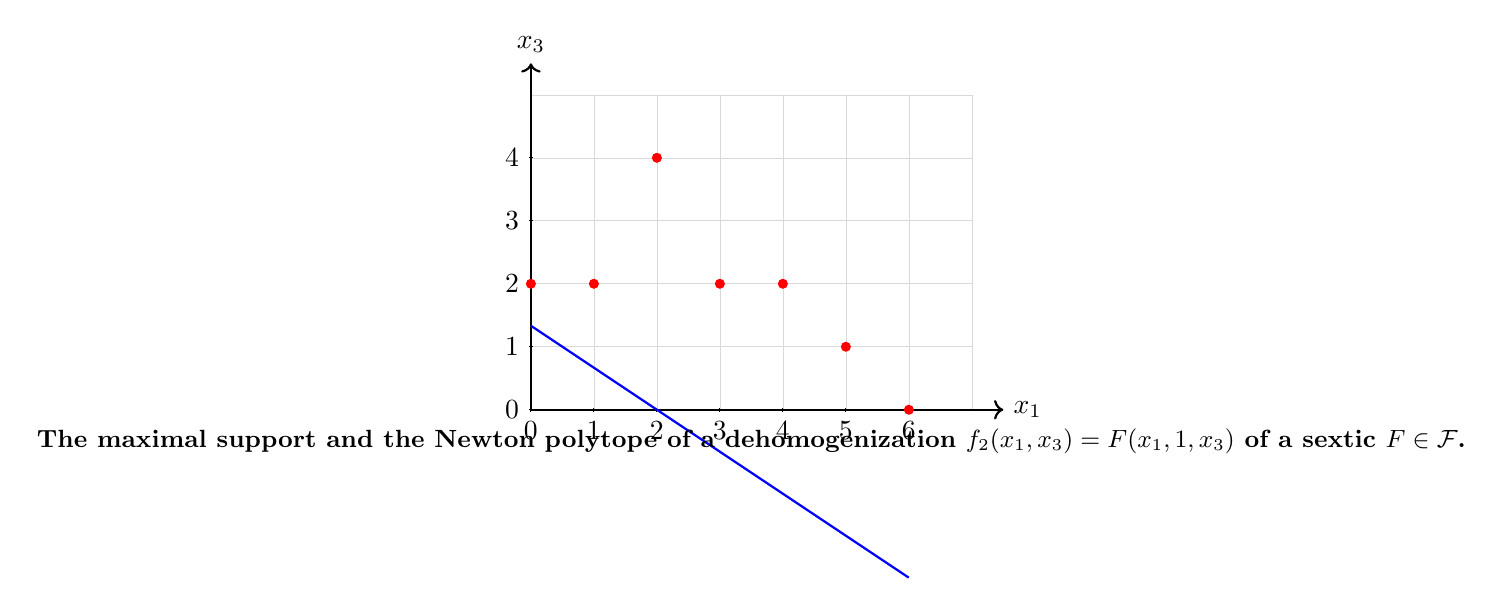
\begin{tikzpicture}[scale=0.8]
    % Grid
    \draw[help lines, color=gray!30] (0,0) grid (7,5);
    
    % Axes
    \draw[->, thick] (0,0) -- (7.5,0) node[right] {$x_1$};
    \draw[->, thick] (0,0) -- (0,5.5) node[above] {$x_3$};
    
    % Labels on axes
    \foreach \x in {0,...,6}
        \draw (\x cm,1pt) -- (\x cm,-1pt) node[anchor=north] {\x};
    \foreach \y in {0,...,4}
        \draw (1pt,\y cm) -- (-1pt,\y cm) node[anchor=east] {\y};
    
    % Plot points
    \filldraw[red] (0,2) circle (2pt);
    \filldraw[red] (1,2) circle (2pt);
    \filldraw[red] (2,4) circle (2pt);
    \filldraw[red] (3,2) circle (2pt);
    \filldraw[red] (4,2) circle (2pt);
    \filldraw[red] (5,1) circle (2pt);
    \filldraw[red] (6,0) circle (2pt);
    
    % Plot line
    \draw[blue, thick, domain=0:6, samples=100] plot (\x,{(4-2*\x)/3});
    
    % Caption
    \node at (3.5,-0.5) {\small \textbf{The maximal support and the Newton polytope of a dehomogenization $f_2(x_1,x_3)=F(x_1,1,x_3)$ of a sextic $F\in \mathcal{F}$.}};
\end{tikzpicture}

\end{document}